\documentclass[a4paper,11pt]{article}

\usepackage{a4wide}
\usepackage[pdftex]{hyperref}
\usepackage[pdftex]{graphicx}
\usepackage[utf8]{inputenc}
\usepackage[ngerman]{babel}
\usepackage[T1]{fontenc}
\usepackage{gensymb}
\usepackage{subfigure}
\usepackage{circuitikz}
\usepackage{tikz}
%\usepackage[adobe-utopia]{mathdesign}

\title{Protokoll: Einf\"uhrungsversuch E1}
\author{Gruppe 5: Byron Worms, Raik Dankworth, Martin Knoll}
\date{17. April 2012}

\begin{document}

\begin{titlepage}
\maketitle
\end{titlepage}

\setcounter{section}{5}
%\section{Versuchsdurchführung und Aufgaben}

\subsection{Schiebewiederstand}

\textbf{Aufbau:}
Der erste Versuch beschäftigt sich mit der Widerstandsmessung, wobei mehrere Messtechniken/- Geräte zum Einsatz kamen. 
Dazu wurde folgender Versuchsaufbau als Grundlage genutzt:

\begin{center}
  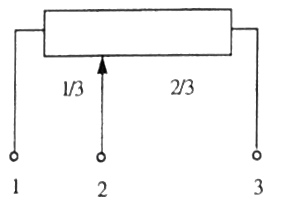
\includegraphics[height=40mm]{51}
\end{center}

Hierbei handelt es ich um einen Schiebewiderstand mit drei möglichen Anschlussstellen für Klemmen. Die zweite Klemme war verschiebbar und sollte in dem Verhältnis 1:2 aus Sicht der ersten Klemme positioniert werden. 

\subsubsection{}

In dem Teilversuch ging es um das Messen von Spannung, Stromstärke und dem daraus resultierenden Widerstand. 
Die dazu benötigten Geräte sind:
\begin{itemize}
  \item Triple Power Supply HM 840
  \item Digitalmultimeter VC 150
  \item Analogmultimeter 2010
\end{itemize}
Hierbei gilt zu beachten, dass man die „Richtigkeit“ für das Messen der jeweiligen Werte einhält. Für die Messung von Spannung muss die Schaltung spannungsrichtig sein, für das Messen der Stromstärke stromrichtig. 

%BILDER Stromrichtig, Spannungsrichtig
\begin{figure}[h!]
  \begin{center}
  \subfigure[spannungsrichtig]{
    \begin{circuitikz}\draw
      (0,2.5)node[left] {$+$} to[short,o-] (0,4)
      to[ammeter] (3,4) -- (5,4)
      to[R] (5,0) -- (3,0)
      (3,4)to[voltmeter] (3,0)
      to(0,0)to[short,-o] (0,1.5) -- (0,1.5)node[left] {$-$};
    \end{circuitikz}
  }
  \subfigure[stromrichtig]{
    \begin{circuitikz}\draw
      (0,2.5)node[left] {$+$} to[short,o-] (0,4)
      to(2,4)to[ammeter] (5,4)
      to[R] (5,0) -- (2,0)
      (2,4)to[voltmeter] (2,0)
      to(0,0)to[short,-o] (0,1.5) -- (0,1.5)node[left] {$-$};
    \end{circuitikz}
  }
\end{center}
\end{figure}

Beide Messungen erfolgten über drei unterschiedliche Kombination der Klemmen: 1-2, 1-3, 2-3.
Daraus resultieren insgesamt 12 Ergebnisse für die Stromstärke und der Spannung. Hinzukommend sind 6 ermittelte Werte für den jeweiligen Widerstand bzgl. der Klemmenkombinationen.  
Es folgen die Ergebnisse unserer Messungen.

\begin{center}
\begin{tabular}{c|rr|rr}
  & \multicolumn{2}{c|}{\textbf{Stromrichtig}}
  & \multicolumn{2}{c}{\textbf{Spannungsrichtig}} \\
  & I in mA & U in V & I in mA & U in V \\
  \hline
  1 - 2 & 250 & 2,497 & 250 & 2,274 \\
  2 - 3 & 250 & 5,169 & 250 &  4,838\\
  1 - 3 & 250 & 7,840 & 250 &  7,420\\
\end{tabular}
\end{center}

Der Widerstand lässt sich wie folgt berechnen:  Spannung[U] / Stromstärke[I]
Man konnte leichte Ungenauigkeiten bei der Messung feststellen. Theoretisch müsste die Addition der Widerstände von 1-2 und 2-3 genau 1-3 ergeben, was praktisch sogut wie nicht erreichbar ist. Dies kann dadurch erklärt werden, dass es keine widerstandslosen Leitung gibt und die Übergänge innerhalb des Schiebewiderstands ebenfalls verlustbehaftet sind. 
Je mehr Kontaktstellen es in einem Versuchsaufbau gibt, desto mehr Störwiderstände müssen erwartet werden. 

\subsubsection{}
Der nächste Teilversuch beschäftigt sich ebenfalls mit Widerstandsmessungen. 
Diesmal wurden drei unterschiedliche Widerstandsmessgeräte eingesetzt und nicht, wie bei der Aufgabe zuvor, der Widerstand per Hand bestimmt. 

Die zu nutzenden Geräte waren folgende:

\begin{itemize}
  \item Digitalmultimeter VC 150
  \item Digitalvoltmeter G-1002.500
  \item Kleinmessbrücke nach Wheatstone
\end{itemize}

Die Messungen lieferten folgende Ergebnisse:

\begin{center}
\begin{tabular}{c|r|r|r}
  & VC 150 (\ohm) & G- 1002.500 (\ohm) & Wheatstone (\ohm) \\
  \hline
  1 - 2 & 26,6 & 26,4 & 27,0 \\
  2 - 3 & 18,2 & 18,2 & 18,3 \\
  1 - 3 & 8,4 & 8,3 & 8,5 \\
\end{tabular}
\end{center}


\subsubsection{}

Hier sollten nun die Widerstände aus 5.1 und 5.2 gegenübergestellt werden. 
Zusätzlich sollte für jede Aufgabe der arithmetische Mittelwert berechnet werden und überprüft werden, ob aus den beiden Teilwiderständen der Gesamtwiderstand berechnet werden kann. 

\begin{center}
\begin{tabular}{c|r|r}
  & Stromrichtig (\ohm) & Spannungsrichtig (\ohm) \\
  \hline
  1 - 2 & 9,988 & 9,096 \\
  2 - 3 & 20,676 & 19,352 \\
  1 - 3 & 31,36 & 29,68 \\
\end{tabular}
\end{center}


Die Unterschiede zwischen den analogen und digitalen gemessenen Widerständen lassen sich wie bei 5.1.1 erklären. 
Bei der analogen Messung  beeinflussen viel mehr Störwiderstände die Genauigkeit. Bei der Digitalen hingegen kommen optimierte und festverdrahtete Schaltungen zum Tragen, die den Störwiderstand auf ein Minimum reduzieren. 
Der Gesamtwiderstand kann nicht durch die beiden einzelnen Teilwiderstände berechnet werden, da die Störwiderstände mehrmals mit einberechnet wurden, was zur Verfälschung des Gesamtwiderstandes führt. 

\subsection{Effektiv- und Spitzenwertmessung}

Bei diesem Versuch ging es um die Spitzenwert- und Effektivmessung. Die Messungen werden nicht mehr mit Gleichstrom, sondern mit Wechselstrom durchgeführt. Der Spitzenwert im Wechselstrom ist die maximale Spannung, die erreicht werden kann bzw. erreicht wird. 
Der Spitzenwert wird von der x-Achse aus bis hin zum Maximalpunkt der Kurve beschrieben. 
Der Effektivwert ist die Durchflussmenge. Diese kann mit Hilfe von Integralrechnungen bestimmt werden, wobei drauf zu achten ist, dass der Betrag der Funktion betrachtet wird. Das Integral wird dabei nur über eine Frequenz berechnet, indem man das berechnete Integral durch Zeit teilt. 
Man kann im Allgemeinen sagen, je höher der Spitzenwert bei gleichbleibender Frequenz ist, desto höher wird auch der Effektivwert. 

Folgende Geräte wurden für den Versuch genutzt:
\begin{itemize}
  \item Function Generator HAMEG HM 8040-4
  \item Analogmultimeter 2010
  \item Digitalmultimeter VC 150
  \item Millivoltmeter MV 21
  \item Oszilloskop HM 203-7
\end{itemize}

Die Messung brachte folgende Werte hervor:
\begin{center}
\begin{tabular}{rrl}
  Analogmultimeter: & 3.6V & (Effektivwert) \\
  Digitalmultimeter: & 3.445V & (Effektivwert) \\
  Millivoltmeter: & 3.6V & (Effektivwert) \\
\end{tabular}
\end{center}

\subsection{Oszillografieren von Sinus- und Rechteckspannungen}

In dem Versuch ging es um die Ermittlung der Frequenzen der Sinus- und Rechtecksfunktion.  

\begin{center}
  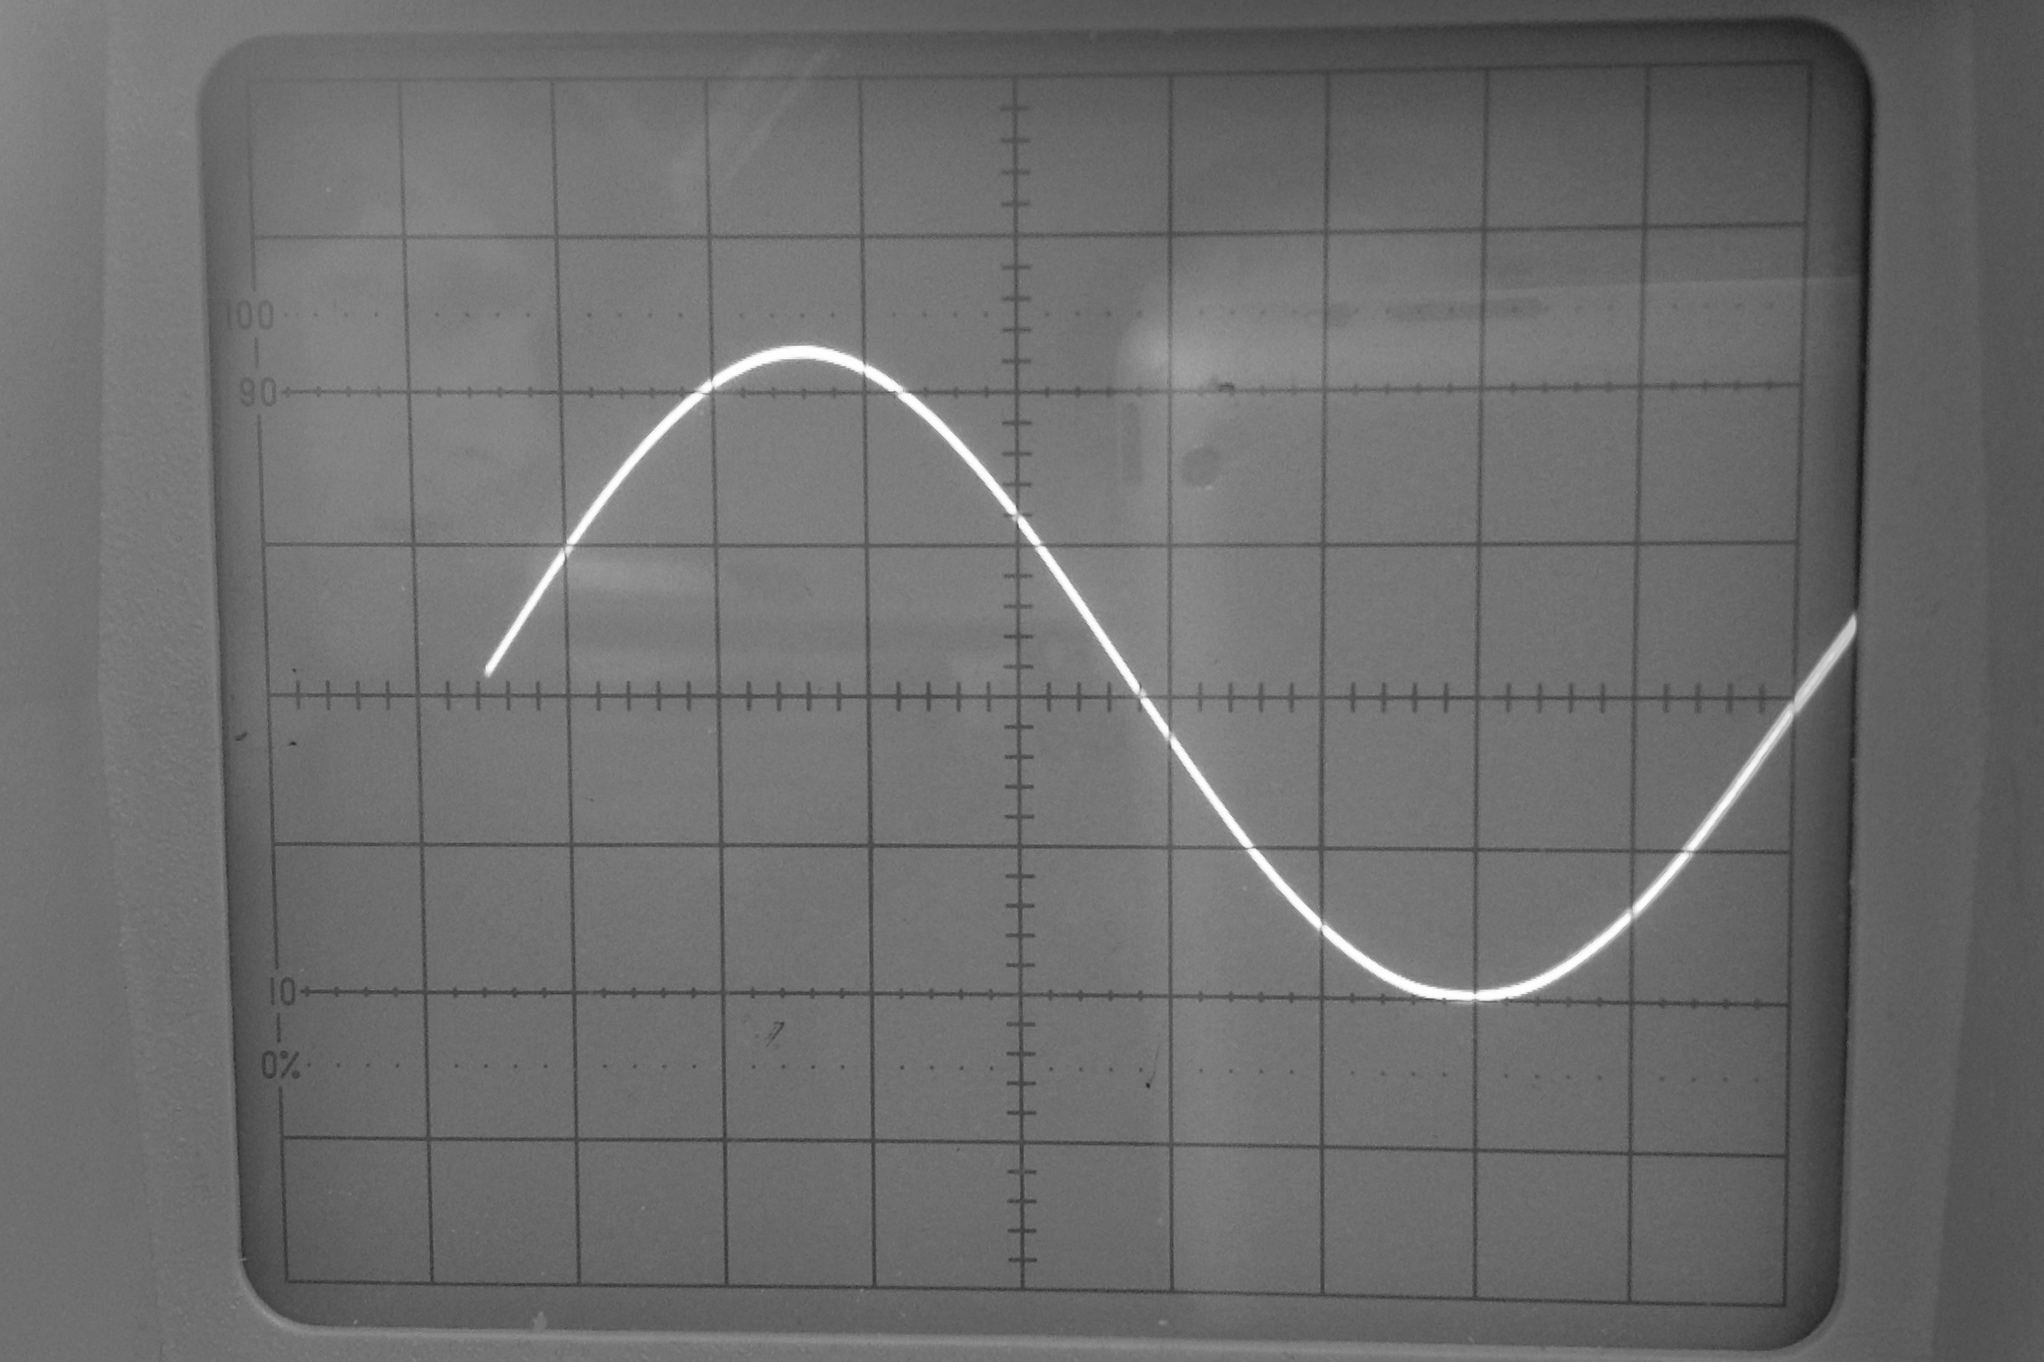
\includegraphics[height=35mm]{Sinus}
  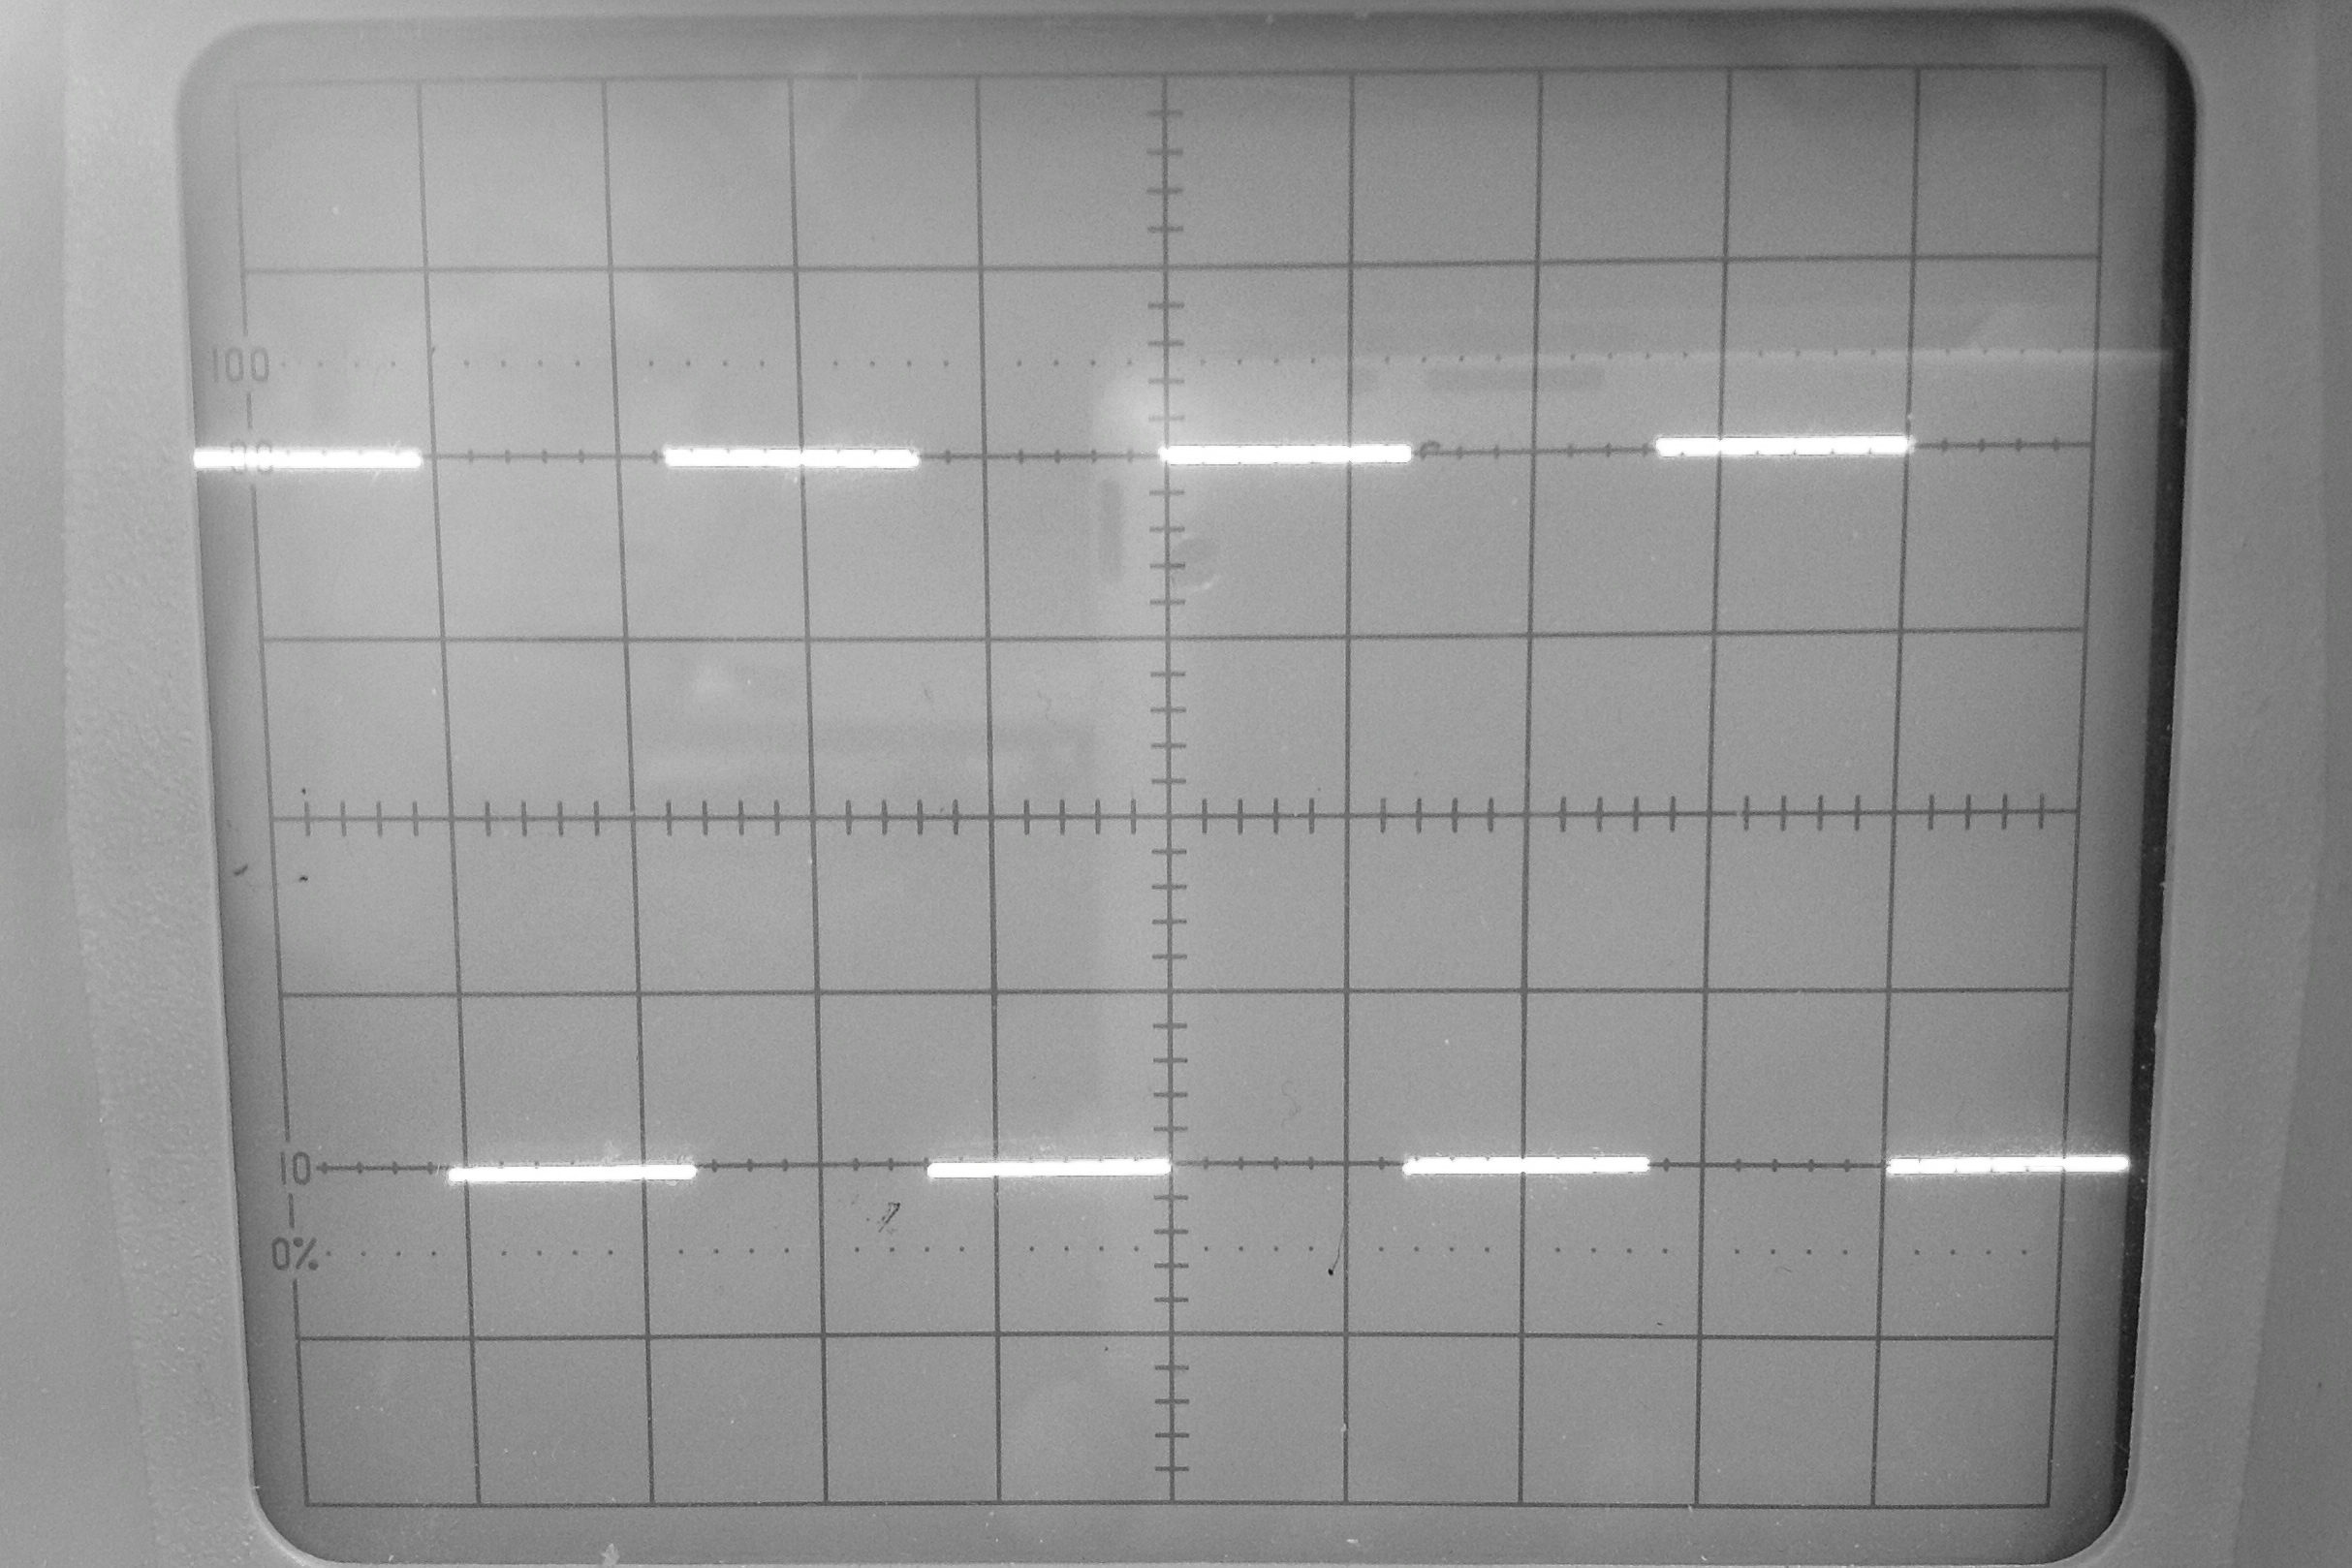
\includegraphics[height=35mm]{Rechteck}
\end{center}

Die Vorgehensweise war für beide Kurven die Gleiche. Als Erstes musste ein Spitzenwert gewählt werden, bei dem das Ablesen eine möglichst gute Genauigkeit liefert. Gewählt wurde von uns beide Male 4 Volt. 
Nachdem man einen passablen Spitzenwert eingestellt hatte, musste die Kurve auf eine gut ablesbare Position auf der x-Achse gebracht werden, sodass man von einer Frequenz die Zeit möglichst genau ablesen konnte. 
Die Zeit von solch einer Frequenz bekommt man ermittelt, indem man die „Kästchen“ in dem Oszillogramm zählte (Anfang der Frequenz bis Ende der Frequenz auf der x-Achse). 

Die Ergebnisse der Messungen sind folgende:

\begin{center}
\begin{tabular}{r|r|r}
  &  gemessen (mhz) & real (mhz) \\
  \hline
  Sinusfunktion & 1136 & 1074 \\
  Rechteckfunktion & 1136 & 1074 \\
\end{tabular}
\end{center}

\subsection{Lissajous-Figuren}

Hierbei sollte eine Frequenzmessung mit Hilfe von Lissajous-Figuren durchgeführt werden. 
Die folgenden Geräte wurden dafür verwendet:
\begin{itemize}
  \item Function Generator HAMEG HM 8030-4 (Sinusspannung)
  \item Tonfrequenzgenerator GF 22
  \item Oszilloskop
\end{itemize}

Das Ziel war es nun bestimmte Frequenzverhältnisse mit Hilfe der beiden Generatoren herzustellen (0.5:1, 1:1, 2:1, 3:1). 
Dazu haben wir den Tonfrequenzgenerator auf 1000 HZ fest eingestellt. Der HAMEG HM 8030-4 wurde dann dementsprechend angepasst, um die Verhältnisse zu erzeugen.   

\begin{figure}[h!]
  \subfigure[0,5:1]{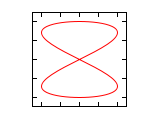
\includegraphics[height=25mm]{12}}
  \subfigure[1:1]{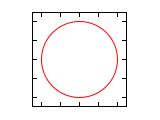
\includegraphics[height=25mm]{11}}
  \subfigure[2:1]{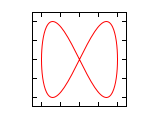
\includegraphics[height=25mm]{21}}
  \subfigure[3:1]{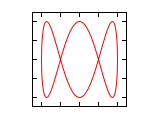
\includegraphics[height=25mm]{31}}
  \\ \centering{\tiny{Quelle: Wikipedia}}
\end{figure}


Mathematisch handelt es sich bei den Lissajous-Kurven um eine parametrische Funktion:

\[
  t \mapsto
  \left(\begin{array}{rr}
    A_x \sin (\omega_1t+\phi_1) \\
    A_y \sin (\omega_2t+\phi_2) \\
  \end{array}\right), 
  t \in [0,\infty]
\]

Diese Funktion ist genau dann periodisch, wenn sich das Frequenzverhältnis sich auf einen ganzzahligen Bruch zurückführen lässt, also rational ist.

\[
  v = \frac{\omega_1}{\omega_2} = \frac{n_1}{n_1}
\]


Die Amplituden Ax und Ay sind nur für die Skalierungen auf horizontaler bzw. vertikaler Ebene da. Das Erscheinungsbild ist hauptsächlich von dem Frequenzverhältnis v und der Phase abhängig. 

Man kann Lissajous-Figuren auf einem Oszilloskop erzeugen, in dem man an den Eingang X und Y eine harmonische Wechselspannung anlegt (Zeitablenkung muss hierbei ausgeschaltet sein.) 

\end{document}
